\section{Problema 3: Escapando}

Luego de juntar todas las piezas, Indy llega a la cruz marcada en el mapa y se encuentra con una red de carritos que parecen dirigirse hacia afuera de la fortaleza, cuando de repente la fortaleza se empieza a derrumbar, así que no tiene mas opción que usar los carritos para escapar.

Los parámetros de entrada son los siguientes:

		\begin{itemize}
		\item Dos números N y M que representan la cantidad de estación y la cantidad de vías
		\item M lineas, las cuales contienen 3 enteros A,B y C que representan que ir de A a B tarda C segundos. Las estaciones se encuentran numeradas desde 1 hasta N
    		\end{itemize}

Los parámetros de salida son los siguientes:

	\begin{itemize}
	\item Un entero T que indica el tiempo mínimo necesario para escapar. En caso de que no haya camino, este valor deberá ser -1
	%\item Asumiendo que haya solución, la siguiente linea contendrá la cantidad de estaciones a recorrer.
	%\item Asumiendo que haya solución. Esta linea deberá contener la secuencia de las estaciones a recorrer.
	\item Si hay solución, la siguiente linea contendrá la cantidad de estaciones a recorrer y la siguiente linea contendrá la secuencia de estaciones a recorrer
	\end{itemize}

La solución tiene que tener una complejidad temporal de $\mathcal{O}(N^{2}log^{2}(N))$ o mejor.

\subsection{Solución}

Vamos a modelar el problema mediante grafos dirigidos. Si pensamos a las estaciones como los vértices y el tiempo necesario para ir de una estación a otra como el peso de la arista dirigida correspondiente, resulta que el problema se reduce a calcular el camino mínimo entre la estación 1 (donde están ubicados) y la estación n , a la cual quieren llegar.

%Si bien parece trivial, no sabemos si hace falta aclararlo.
La longitud del camino es la sumatoria de las aristas que usa, por lo dicho anteriormente esto equivale al tiempo necesario para recorrer dicho camino, esto seria la primera linea de la salida.

Para poder devolver la secuencia, vamos a tener un array de predecesores, que contendrá para todo los nodos del camino solución, desde qué nodo llegué.

Para resolver el problema vamos a aplicar un algoritmo de camino mínimo en grafos, en este caso vamos a usar Dijkstra, ya que todas las aristas tienen peso positivo.

\begin{lstlisting}
    $visitados$ $\gets$ vector[n,false]
    $tiempo\_min$ $\gets$ vector[n, $\infty$]
    $padre$ $\gets$ vector[n,-1]

    $tiempoMin$[0] = 0

    while $true$:
        $estacion\_actual$ $\gets$ $-1$
        $tiempo\_actual$ $\gets$ $\infty$

        for $j$ in [0..n) do
            If $j$ no fue visitado y $tiempo\_min$[$j$] < $tiempo\_actual$
                $estacion\_actual$ = $j$
                $tiempo\_actual$ = $tiempo\_min$[j]
        Si no encontre un candidato sin visitar y con $tiempo\_min$ $\neq \infty$
            break

        Marco el $nodo\_actual$ como visitado

        Si es el nodo buscado
            return el tiempo necesario

        for $a$ in lista de adyacencia de $nodo\_actual$
            $tiempo\_nuevo$ $\gets$ a $a$ desde $nodo\_actual$
            Si $tiempo\_nuevo$ < $tiempo\_min$[$a$]:
                actualizo el $tiempo\_min$[$a$]
                actualizo el padre de $a$

    return -1
   \end{lstlisting}

\subsection{Correctitud}

La demostración del algoritmo se vio en las clases teóricas de la materia.

\subsection{Complejidad}
Antes que nada, tenemos que inicializar las estructuras que vamos a utilizar.

Generar los 3 arrays visitados,TiempoMin y padre, lleva tiempo lineal en la cantidad de entradas, hay que pedir la memoria y luego recorrer linealmente cada array para insertar el valor que queremos. Como cada array tiene N elementos, donde N es la cantidad de estaciones,  esto tiene costo $\mathcal{O}(N)$

Luego tenemos un ciclo,  veamos su costo.

Buscar cual va a ser el siguiente nodo visitado es lineal ya que  recorreremos  todo el arreglo y vamos  comparando. Cabe aclarar que dentro de esta parte solo se comparan enteros y bool que se realiza en tiempo constante.. Por lo tanto esto tiene costo $\mathcal{O}(N)$

Luego se hacen 2 comparaciones, una para detectar el caso de que no pueda seguir y no haya solución y la otra para ver si encontré el nodo buscado. Estas comparaciones, se realizan en tiempo constante pues es comparar 1 entero en cada una. $\mathcal{O}(1)$

Luego,  sigue un for que itera sobre los vecinos del nodo actual . Este for tiene un costo lineal en la cantidad de vecinos del nodo, ya que lo de adentro se puede acotar por una constante.  Dado que no podemos asumir cotas inferiores para la cantidad de vecinos, el peor caso , cada nodo es vecino de todos, este for tiene costo  $\mathcal{O}(N)$

Todo este ciclo se realiza mientras no tengamos el camino mínimo  hasta el nodo N.  En caso de que exista un camino este ciclo se ejecuta a lo sumo N veces y en el caso de que no exista también se ejecuta a lo sumo N veces, ya que realiza (K) ejecuciones completas donde K es la cantidad de nodos alcanzables desde el origen y luego entra 1 vez mas, realiza el primer for y sale por el break. Este K esta acotado por N-1.

Por lo tanto tenemos un ciclo que se ejecuta a lo sumo N veces y el ciclo tiene costo $\mathcal{O}(N)$. Por lo tanto nuestro algoritmo tiene costo $\mathcal{O}(N^{2})$.


\subsection{Experimentación}

Para realizar la experimentación escribimos cuatro generadores de grafos que toman como entrada la cantidad de nodos requerida.

\begin{itemize}

    \item Generador completo: Crea un digrafo completo con $n$ nodos, y pesos de aristas aleatorios entre 1 y 1000

    \item Generador random: Crea un digrafo completo con $n$ nodos y pesos de aristas aleatorios entre 1 y 1000, y para cada arista decide si borrarla con una probabilidad de 0.5

    \item Generador ciclo: Crea una arista de cada nodo $i$ al nodo $i+1$ (para $i$ < n) y otra del último al primero, con peso aleatorio entre 1 y 1000

    \item Generador grilla: Crea una grilla de $\lfloor \sqrt{n} \rfloor \times \lfloor \sqrt{n} \rfloor$ donde cada nodo está conectado con sus cuatro vecinos con una arista de peso aleatorio entre 1 y 1000. Los $n \mod \lfloor \sqrt{n} \rfloor$ restantes tienen una arista incidente desde el nodo anterior de peso aleatorio

\end{itemize}

En los primeros dos generadores podemos ver que la cantidad de aristas será \bigo($n^2$), ya que el grafo completo tendrá en total $n * (n-1)$ aristas y el grafo random aproximadamente la mitad.

En cambio, el grafo ciclo es casi el grafo conexo mas simple que podemos generar, con exactamente $n$ aristas.

El grafo grilla tendrá aproximadamente $4$ arcos saliendo de cada nodo de la grilla (excepto en los bordes) y luego $n \mod \lfloor \sqrt{n} \rfloor$ aristas extra. Como la grilla tiene $\lfloor \sqrt{n} \rfloor^2 \simeq n$ nodos, la cantidad final sera \bigo($n$).

    \begin{figure}[H]
    	\centering
    	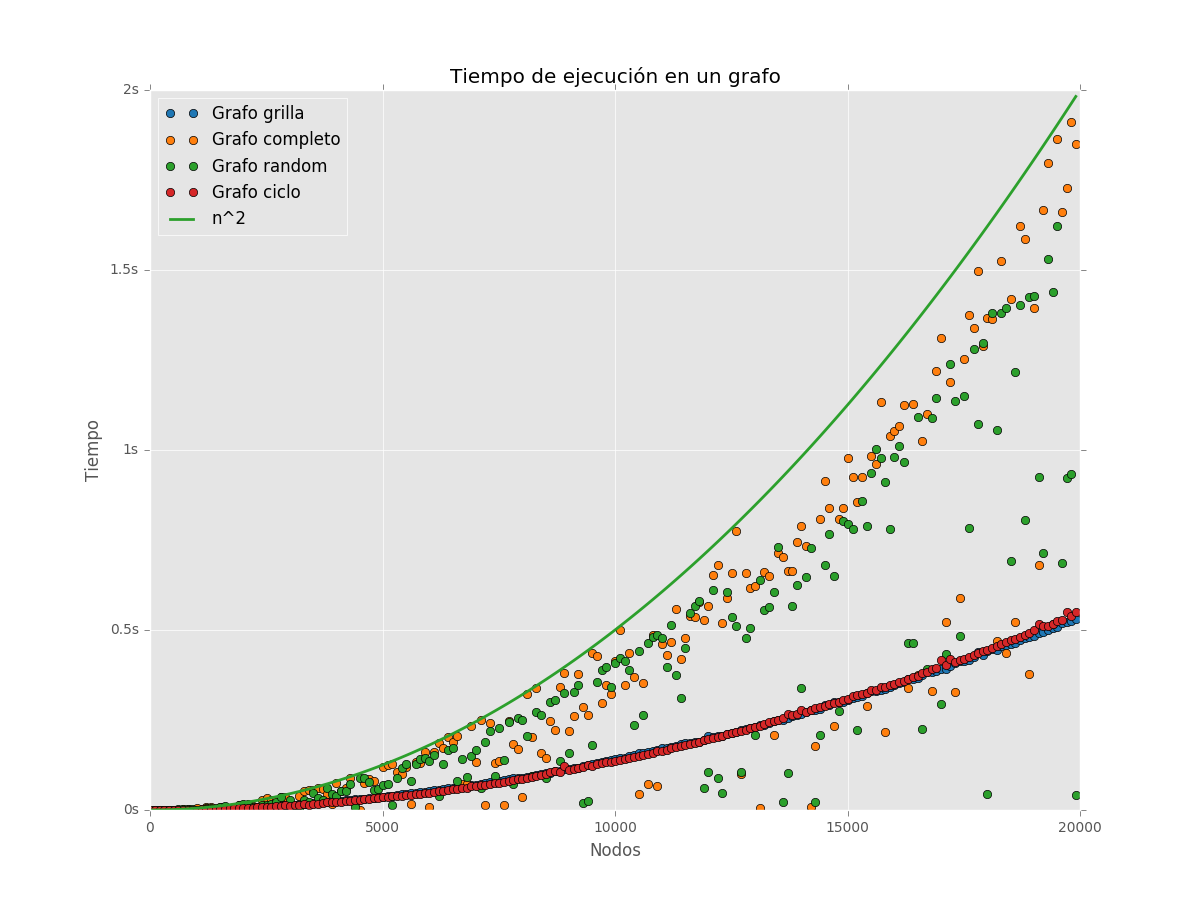
\includegraphics[width=\textwidth]{ej3-all}
    	\caption{Tiempo de ejecución del problema 3 usando diferentes generadores de grafos con $n$ nodos}
    	\label{fig:ej3-all}
    \end{figure}

En la figura \ref{fig:ej3-all} podemos apreciar el comportamiento cuadrático del algoritmo, independientemente del orden de la cantidad de aristas. Más aún, se pueden discernir bastante bien
los diferentes tiempos de ejecución para cada grafo definido anteriormente. Por ejemplo, los generados como completos tienen cantidad máxima de aristas y son los que más cercanos a la cota superior se mantienen (tienen que actualizar más vecinos en peor caso), aunque hay casos de bajo tiempo de ejecución que suceden cuando el algoritmo encuentra temprano una arista muy liviana hacia el punto de salida. El random, al construirse sobre el completo, presenta una dispersión similar. Distinto es el caso para el grilla o el ciclo, donde ambos marcan una curva perfectamente definida (en el gráfico las corridas sobre ciclos (rojas) solapan un poco las del grilla (azules)). Esto se debe a que cada vecino tiene una cantidad $\mathcal{O}(1)$ de vecinos y por lo tanto, cuando actualizamos vecinos, lo haremos una cantidad constante de veces en peor caso para cada nodo versus la cota $\mathcal{O}(n)$ que teníamos para el caso general. En el caso del grilla, cada nodo tiene a lo sumo 4 vecinos, y en el ciclo tienen 2.
